\documentclass[twoside]{article}
\usepackage{supertabular}
\usepackage{array}
\usepackage{multicol}
\usepackage{graphicx}
\usepackage[textwidth=20cm,textheight=24cm]{geometry}
\usepackage{hhline}
\usepackage{fontspec}
\setmainfont{Calibri}
\usepackage[table, dvipsnames]{xcolor}
\usepackage{multirow}
\usepackage{boldline}
\usepackage{dcolumn}
\newcolumntype{d}[1]{D{.}{.}{ #1 }}

\definecolor{myblue1}{RGB}{141,179, 226}
\definecolor{myblue2}{RGB}{79,129, 189}
\definecolor{myblue3}{RGB}{74,126, 187}
\definecolor{mykhaki}{RGB}{168,177, 148}
\newcommand{\thiscolor}[1]{\texttt{ #1 } \hfill \fcolorbox{black}{ #1 }{\hspace{2mm}}}
\setlength{\headheight}{15pt}
\usepackage{fancyhdr}
\pagestyle{fancy}
\fancyhf{}
\fancyhead[C]{\small \textcolor{mykhaki} {Proyecto Colibrí de la Montaña }}
\fancyhead[LO,LE]{\small \textcolor{mykhaki} {Manifestación de Impacto Ambiental modalidad regional}}
\fancyhead[RE,RO]{\begin{tabular}{cc}\small \textcolor{mykhaki} {Capítulo 2  (Sección II)} & \small \textcolor{mykhaki} { Pág. \thepage}\end{tabular}}
\usepackage{xpatch}
\xpretocmd\headrule{\color{mykhaki}}{}{\PatchFailed}





\begin{document}
\begin{flushleft}
\tablefirsthead{}
\tablehead{}
\tabletail{}
\tablelasttail{}
\arrayrulecolor{myblue3}

\begin{tabular}{m{7.7320004cm}m{0.091000006cm}|m{2.421cm}|m{0.089cm}m{0.694cm}m{0.693cm} m{0.703cm}m{0.703cm}m{0.703cm}m{0.703cm}m{0.703cm} }
\hhline{ ~~-~~~~~~~~ }
 ~&~ & \multirow{2}{*}{\centering\textcolor{myblue2}{Clave: PUEB}}&~ &\footnotesize Etapa:&\footnotesize\textcolor{myblue2} {\textbf{ 2 }} &~&~&~&~&~
\\\hhline{ ~~~~~-----~ }
\textcolor{myblue2} {Módulo:}&~& &~&\multicolumn{1}{m{0.694cm}|}{\footnotesize Años: } &

  \multicolumn{1}{m{0.693cm}|}{  \footnotesize\centering 1-5  } &

  \multicolumn{1}{m{0.693cm}|}{ \cellcolor{gray!50} \footnotesize\centering 6-15  } &

  \multicolumn{1}{m{0.693cm}|}{  \footnotesize\centering 16-17  } &

  \multicolumn{1}{m{0.693cm}|}{  \footnotesize\centering 18-20  } &

  \multicolumn{1}{m{0.693cm}|}{  \footnotesize\centering 21-99  } &

~
\\\hhline{ ~~-~~-----~ }
\textcolor{myblue2} { Pueblito }
 &~& \cellcolor{myblue1}\footnotesize\centering\color{white}\textbf{ Construcción }
 &~&

\multicolumn{ 7 }{l}{\footnotesize Duración de la obra o actividad: \textcolor{myblue2} {\textbf{ 1,457 días en 10 años}}}


\\\hhline{ ~~-~~~~~~~~ }

\end{tabular}
\end{flushleft}

{\color{myblue2} \rule{\linewidth}{0.6mm} }

\begin{multicols}{2}

\bigskip

\footnotesize\textcolor{myblue2} {\textbf{ Localización}}


\bigskip

 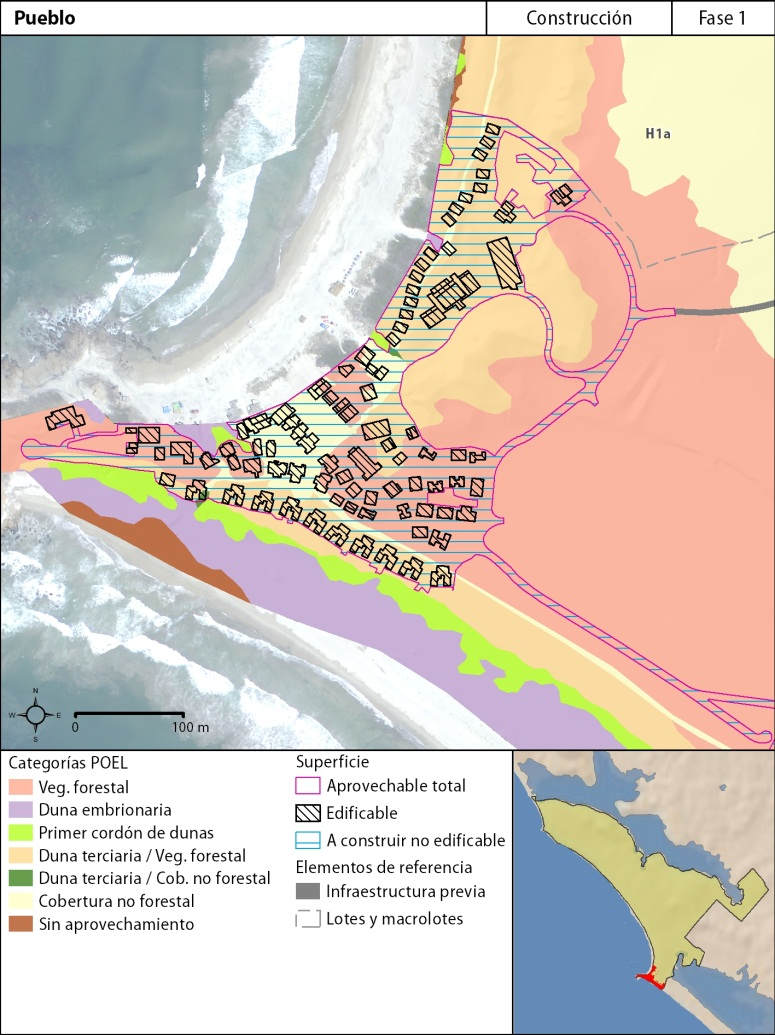
\includegraphics{C:/Users/arabela/Documents/GitHub/cap2/test_latex_templates/img/img001.jpg}


\bigskip


\bigskip

\footnotesize Categorías del POEL: Duna embrionaria (DEM); dunas terciarias/vegetación forestal (DTF); dunas terciarias/cobertura no forestal (DTN); dunas terciarias/vegetación secundaria de selva (DTS); primer cordón de dunas (PCD); selva baja caducifolia (SBC); vegetación forestal (VFO); cobertura no forestal (CNF); vegetación secundaria de selva (VSS).


\bigskip


\bigskip

\textcolor{myblue2} {\textbf{Descripción general del componente para esta fase}}


\bigskip

\footnotesize El componente “Pueblo” se construirá a lo largo de dos fases (años 1 al 10) e integrará edificaciones relacionadas con actividades hoteleras y residenciales, actividades sociales, deportivas, artísticas y culturales, actividades comerciales y de servicios, pesca y venta de productos frescos del mar.

La fase 1 incluirá la construcción de dos hoteles boutique así como múltiples villas residenciales para alojar a visitantes (véase la tabla Construcción de producto inmobiliario para esta fase), familias de pescadores locales, trabajadores y operadores del condominio. Para las actividades comerciales y de servicios se construirán 25 edificaciones consistentes en tres restaurantes, cuatro mercados de misceláneos y productos del mar, siete comercios de productos diversos, una capilla, un módulo de escamoche, almacén y lavado de pescado, dos bodegas de refrigeración, un módulo de baños públicos y bodega, cinco establecimientos de servicios varios tales como un consultorio de atención médica de primer contacto, delegación municipal, una lavandería y dos oficinas. Para las actividades recreativas y culturales, en esta fase se construirá un gimnasio. Se construirá un estacionamiento para facilitar el ingreso a los hoteles boutique y áreas aledañas.

La totalidad de las edificaciones de este componente se clasificarán en dos sistemas constructivos: palafitos y edificación convencional (ver sistemas constructivos al final de este apartado), y respetarán una altura máxima de 8 m o dos niveles (incluyendo la planta baja y tomando en cuenta la altura a nivel de piso natural) para mantener la visibilidad hacia la costa; de acuerdo a lo que establece el POEL en relación a las edificaciones que se ubiquen a una distancia menor a 200 m de la Zona Federal Marítimo Terrestre.

La ubicación donde se desplantará este componente coincide con la actual localización del punto público de acceso vehicular a la playa, en donde existe un asentamiento humano de familias de pescadores conformado por seis palapas o enramadas, donde viven itinerantemente alrededor de 12 familias (ver Medidas de responsabilidad social).

Además, en este sitio se encuentra la infraestructura que actualmente alberga las instalaciones del Campamento de Conservación de Tortugas Marinas administrado por la Comisión Nacional de Áreas Naturales Protegidas (CONANP) en Chalacatepec. Dicha infraestructura será remplazada por instalaciones nuevas y diseñada de acuerdo al programa de necesidades apegado a los requerimientos de la normatividad ambiental vigente; para tal efecto, será necesario demoler las actuales (ver Demolición de las instalaciones del actual Campamento Tortuguero) y el Campamento será reubicado con la finalidad de mejorar las condiciones constructivas y operativas de las actuales instalaciones.

Además de la superficie edificable, como parte de las áreas exteriores del componente se construirán vialidades secundarias y estacionamientos de empedrado asentado en arena (ver Sistema constructivo de vialidades secundarias convencionales); terrazas y explanadas, áreas verdes ornamentales y deportivas, dos albercas y diversos andadores de acceso al mar; todo esto empleando sistemas constructivos convencionales.

Se construirán las redes secundarias de infraestructura hidráulica, sanitaria y de agua tratada requeridas para garantizar el abastecimiento de agua potable y la conducción del agua residual hacia su proceso de tratamiento, y desde el mismo, de vuelta a su origen para ser reutilizada en el riego de áreas verdes ornamentales. El componente cuenta con su propia Planta de Tratamiento al interior del mismo (ver componente Plantas de Tratamiento de aguas residuales y manejo de aguas residuales) y una línea de descarga de excedentes de agua tratada hasta un estanque artificial.

Se construirán además las obras secundarias de infraestructura eléctrica de baja tensión y de telecomunicaciones. La siguiente tabla muestra la totalidad de las redes de infraestructura a implementarse en esta fase.
\bigskip


\begin{tabular}{ |p{ 5cm }|d{2.1}|d{2.1}|d{2.1}|}
\hline
\multicolumn{ 4 }{|l|}{\cellcolor{myblue1}\scriptsize\color{white}{ Longitudes de infraestructura a implementar por categoría del POEL (km) }}\\
\hline
\multicolumn{1}{ |c|}{\scriptsize\textcolor{myblue2} { Tipo de red } } & \multicolumn{1}{ c|}{\scriptsize\textcolor{myblue2} { VFO } } & \multicolumn{1}{ c|}{\scriptsize\textcolor{myblue2} { DTF } } & \multicolumn{1}{ c|}{\scriptsize\textcolor{myblue2} { CNF } } & 
\hline


\scriptsize Hidráulica &

\scriptsize 1.4 &

\scriptsize 0.3 &

\scriptsize 0.2 &

\hline


\scriptsize Sanitaria &

\scriptsize 1.4 &

\scriptsize 0.4 &

\scriptsize 0.2 &

\hline


\scriptsize Agua tratada &

\scriptsize 1.6 &

\scriptsize 0.4 &

\scriptsize 0.2 &

\hline


\scriptsize Telecomunicaciones &

\scriptsize 1.2 &

\scriptsize 0.6 &

\scriptsize 0.2 &

\hline


\scriptsize Eléctrica aérea &

\scriptsize 0.2 &

\scriptsize 0 &

\scriptsize 0.1 &

\hline


\scriptsize Eléctrica subterránea &

\scriptsize 1.0 &

\scriptsize 0.5 &

\scriptsize 0.3 &

\hline


\end{tabular}

\bigskip

Previo al inicio de los procesos de obra, las actividades del componente incluyen la construcción de edificaciones de carácter provisional denominadas Obras temporales, las cuales se ubicarán en la brecha existente que bordea el componente al límite sureste así como en el sitio donde será la explanada central del componente el cual presenta Cobertura No Forestal; dichos espacios tendrán la finalidad de servir como áreas auxiliares de trabajo y almacenamiento desde donde los trabajadores se desplazarán al lugar de trabajo corres-pondiente. Estas obras no formarán parte del componente pero son necesarias para alber-gar de forma temporal trabajadores, insumos, maquinaria, equipos, etc.; y serán retiradas una vez concluida la totalidad del componente al término de la fase 2.

\bigskip

\footnotesize El componente “Pueblo” se construirá a lo largo de dos fases (años 1 al 10) e integrará edificaciones relacionadas con actividades hoteleras y residenciales, actividades sociales, deportivas, artísticas y culturales, actividades comerciales y de servicios, pesca y venta de productos frescos del mar.

La fase 1 incluirá la construcción de dos hoteles boutique así como múltiples villas residenciales para alojar a visitantes (véase la tabla Construcción de producto inmobiliario para esta fase), familias de pescadores locales, trabajadores y operadores del condominio. Para las actividades comerciales y de servicios se construirán 25 edificaciones consistentes en tres restaurantes, cuatro mercados de misceláneos y productos del mar, siete comercios de productos diversos, una capilla, un módulo de escamoche, almacén y lavado de pescado, dos bodegas de refrigeración, un módulo de baños públicos y bodega, cinco establecimientos de servicios varios tales como un consultorio de atención médica de primer contacto, delegación municipal, una lavandería y dos oficinas. Para las actividades recreativas y culturales, en esta fase se construirá un gimnasio. Se construirá un estacionamiento para facilitar el ingreso a los hoteles boutique y áreas aledañas.

La totalidad de las edificaciones de este componente se clasificarán en dos sistemas constructivos: palafitos y edificación convencional (ver sistemas constructivos al final de este apartado), y respetarán una altura máxima de 8 m o dos niveles (incluyendo la planta baja y tomando en cuenta la altura a nivel de piso natural) para mantener la visibilidad hacia la costa; de acuerdo a lo que establece el POEL en relación a las edificaciones que se ubiquen a una distancia menor a 200 m de la Zona Federal Marítimo Terrestre.

La ubicación donde se desplantará este componente coincide con la actual localización del punto público de acceso vehicular a la playa, en donde existe un asentamiento humano de familias de pescadores conformado por seis palapas o enramadas, donde viven itinerantemente alrededor de 12 familias (ver Medidas de responsabilidad social).

Además, en este sitio se encuentra la infraestructura que actualmente alberga las instalaciones del Campamento de Conservación de Tortugas Marinas administrado por la Comisión Nacional de Áreas Naturales Protegidas (CONANP) en Chalacatepec. Dicha infraestructura será remplazada por instalaciones nuevas y diseñada de acuerdo al programa de necesidades apegado a los requerimientos de la normatividad ambiental vigente; para tal efecto, será necesario demoler las actuales (ver Demolición de las instalaciones del actual Campamento Tortuguero) y el Campamento será reubicado con la finalidad de mejorar las condiciones constructivas y operativas de las actuales instalaciones.

Además de la superficie edificable, como parte de las áreas exteriores del componente se construirán vialidades secundarias y estacionamientos de empedrado asentado en arena (ver Sistema constructivo de vialidades secundarias convencionales); terrazas y explanadas, áreas verdes ornamentales y deportivas, dos albercas y diversos andadores de acceso al mar; todo esto empleando sistemas constructivos convencionales.

Se construirán las redes secundarias de infraestructura hidráulica, sanitaria y de agua tratada requeridas para garantizar el abastecimiento de agua potable y la conducción del agua residual hacia su proceso de tratamiento, y desde el mismo, de vuelta a su origen para ser reutilizada en el riego de áreas verdes ornamentales. El componente cuenta con su propia Planta de Tratamiento al interior del mismo (ver componente Plantas de Tratamiento de aguas residuales y manejo de aguas residuales) y una línea de descarga de excedentes de agua tratada hasta un estanque artificial.

Se construirán además las obras secundarias de infraestructura eléctrica de baja tensión y de telecomunicaciones. La siguiente tabla muestra la totalidad de las redes de infraestructura a implementarse en esta fase.

\bigskip

\begin{tabular}{ |p{ 7cm }|d{2.1}|}
\hline
\multicolumn{ 2 }{|l|}{\cellcolor{myblue1}\scriptsize\color{white}{ Frecuencia de actividades de obras provisionales }}\\
\hline
\multicolumn{1}{ |c|}{\scriptsize\textcolor{myblue2} { Actividades } } & \multicolumn{1}{ c|}{\scriptsize\textcolor{myblue2} { Jornadas/fase } } & 
\hline


\scriptsize Recepción y distribución de insumos &

\scriptsize 1457 &

\hline


\scriptsize Administración de las instalaciones &

\scriptsize 1457 &

\hline


\scriptsize Limpieza y revisión de las instalaciones, incluye: talleres, bodegas y casetas; revisión de muebles de baño como lavabos, inodoro, coladeras, así como grifos y cañerías &

\scriptsize 625 &

\hline


\scriptsize Almacenamiento de equipos, maquinaria, refacciones y herramienta &

\scriptsize 1457 &

\hline


\scriptsize Descanso, preparación y alimentación del personal &

\scriptsize 182 &

\hline


\scriptsize Limpieza general y recolección de residuos y aguas residuales &

\scriptsize 273 &

\hline


\scriptsize Vigilancia de las instalaciones &

\scriptsize 4372 &

\hline


\scriptsize Mantenimiento de áreas de circulación, patios y áreas exteriores. &

\scriptsize 31 &

\hline


\scriptsize Revisión y limpieza de las instalaciones y equipos de cocina &

\scriptsize 5 &

\hline


\scriptsize Mantenimiento menor de maquinaria &

\scriptsize 165 &

\hline


\end{tabular}

\bigskip

Previo al inicio de los procesos de obra, las actividades del componente incluyen la construcción de edificaciones de carácter provisional denominadas Obras temporales, las cuales se ubicarán en la brecha existente que bordea el componente al límite sureste así como en el sitio donde será la explanada central del componente el cual presenta Cobertura No Forestal; dichos espacios tendrán la finalidad de servir como áreas auxiliares de trabajo y almacenamiento desde donde los trabajadores se desplazarán al lugar de trabajo corres-pondiente. Estas obras no formarán parte del componente pero son necesarias para alber-gar de forma temporal trabajadores, insumos, maquinaria, equipos, etc.; y serán retiradas una vez concluida la totalidad del componente al término de la fase 2.

\bigskip

\begin{tabular}{ |p{ 7cm }|c|}
\hline
\multicolumn{ 2 }{|l|}{\cellcolor{myblue1}\scriptsize\color{white}{ Datos generales del componente para esta fase }}\\
\hline


\scriptsize Superficie edificable (ha) &

\scriptsize 1.3 &

\hline


\scriptsize Superficie a construir no edificable (ha) &

\scriptsize 5.45 &

\hline


\scriptsize Macrolotes del plan maestro &

\scriptsize Pueblo &

\hline


\scriptsize UGA POEL &

\scriptsize 101, 151 &

\hline


\scriptsize Niveles máximos construidos &

\scriptsize 2 &

\hline


\scriptsize Cuartos totales construidos &

\scriptsize 150 &

\hline

\end{tabular}

\bigskip

Previo al inicio de los procesos de obra, las actividades del componente incluyen la construcción de edificaciones de carácter provisional denominadas Obras temporales, las cuales se ubicarán en la brecha existente que bordea el componente al límite sureste así como en el sitio donde será la explanada central del componente el cual presenta Cobertura No Forestal; dichos espacios tendrán la finalidad de servir como áreas auxiliares de trabajo y almacenamiento desde donde los trabajadores se desplazarán al lugar de trabajo corres-pondiente. Estas obras no formarán parte del componente pero son necesarias para alber-gar de forma temporal trabajadores, insumos, maquinaria, equipos, etc.; y serán retiradas una vez concluida la totalidad del componente al término de la fase 2.

\bigskip

\begin{tabular}{ |p{ 2.4cm }|p{ 4cm }|c|}
\hline
\multicolumn{ 3 }{|l|}{\cellcolor{myblue1}\scriptsize\color{white}{ Implementación de procesos constructivos por tipo de ecosistema }}\\
\hline
\multicolumn{1}{ |c|}{\scriptsize\textcolor{myblue2} { Proceso constructivo } } & \multicolumn{1}{ c|}{\scriptsize\textcolor{myblue2} { Categoría del POEL } } & \multicolumn{1}{ c|}{\scriptsize\textcolor{myblue2} { Superficie (ha) } } & 
\hline

\multirow{ 4 }{ 2.4cm }{\scriptsize Palafitos } &
    
    
      
      
        \scriptsize Vegetación forestal &
      
        \scriptsize 0.29 &
      
      
        \hhline{|~|-|-| }
      
    
      
       ~  &
      
      
        \scriptsize Duna Terciaria Vegetación forestal &
      
        \scriptsize 0.47 &
      
      
        \hhline{|~|-|-| }
      
    
      
       ~  &
      
      
        \scriptsize Duna Terciaria Cobertura no forestal &
      
        \scriptsize 0 &
      
      
        \hhline{|~|-|-| }
      
    
      
       ~  &
      
      
        \scriptsize Cobertura no forestal &
      
        \scriptsize 0.24 &
      
      
    
    \hline

\multirow{ 3 }{ 2.4cm }{\scriptsize Edificaciones convencionales } &
    
    
      
      
        \scriptsize Vegetación forestal &
      
        \scriptsize 0.27 &
      
      
        \hhline{|~|-|-| }
      
    
      
       ~  &
      
      
        \scriptsize Duna Terciaria Vegetación forestal &
      
        \scriptsize 0.02 &
      
      
        \hhline{|~|-|-| }
      
    
      
       ~  &
      
      
        \scriptsize Cobertura no forestal &
      
        \scriptsize 0 &
      
      
    
    \hline

\multirow{ 3 }{ 2.4cm }{\scriptsize Vialidades secundarias } &
    
    
      
      
        \scriptsize Vegetación forestal &
      
        \scriptsize 0.98 &
      
      
        \hhline{|~|-|-| }
      
    
      
       ~  &
      
      
        \scriptsize Duna Terciaria Vegetación forestal &
      
        \scriptsize 0.31 &
      
      
        \hhline{|~|-|-| }
      
    
      
       ~  &
      
      
        \scriptsize Cobertura no forestal &
      
        \scriptsize 0.13 &
      
      
    
    \hline

\multirow{ 2 }{ 2.4cm }{\scriptsize Albercas convencionales } &
    
    
      
      
        \scriptsize Duna Terciaria Vegetación forestal &
      
        \scriptsize 0.01 &
      
      
        \hhline{|~|-|-| }
      
    
      
       ~  &
      
      
        \scriptsize Cobertura no forestal &
      
        \scriptsize 0.01 &
      
      
    
    \hline

\scriptsize Cuerpo de agua artificial &
    
    
      
      
        \scriptsize Vegetación forestal &
      
        \scriptsize 0.02 &
      
      
    
    \hline

\multirow{ 4 }{ 2.4cm }{\scriptsize Áreas verdes ornamentales } &
    
    
      
      
        \scriptsize Vegetación forestal &
      
        \scriptsize 0.06 &
      
      
        \hhline{|~|-|-| }
      
    
      
       ~  &
      
      
        \scriptsize Duna Terciaria Vegetación forestal &
      
        \scriptsize 0.09 &
      
      
        \hhline{|~|-|-| }
      
    
      
       ~  &
      
      
        \scriptsize Duna Terciaria Cobertura no forestal &
      
        \scriptsize 0 &
      
      
        \hhline{|~|-|-| }
      
    
      
       ~  &
      
      
        \scriptsize Cobertura no forestal &
      
        \scriptsize 0.03 &
      
      
    
    \hline

\multirow{ 4 }{ 2.4cm }{\scriptsize Terrazas, patios y explanadas } &
    
    
      
      
        \scriptsize Vegetación forestal &
      
        \scriptsize 1.38 &
      
      
        \hhline{|~|-|-| }
      
    
      
       ~  &
      
      
        \scriptsize Duna Terciaria Vegetación forestal &
      
        \scriptsize 1.65 &
      
      
        \hhline{|~|-|-| }
      
    
      
       ~  &
      
      
        \scriptsize Duna Terciaria Cobertura no forestal &
      
        \scriptsize 0.01 &
      
      
        \hhline{|~|-|-| }
      
    
      
       ~  &
      
      
        \scriptsize Cobertura no forestal &
      
        \scriptsize 0.49 &
      
      
    
    \hline

\multirow{ 4 }{ 2.4cm }{\scriptsize Instalación hidrosanitaria y de agua tratada secundaria } &
    
    
      
      
        \scriptsize Vegetación forestal &
      
        \scriptsize 0 &
      
      
        \hhline{|~|-|-| }
      
    
      
       ~  &
      
      
        \scriptsize Duna Terciaria Vegetación forestal &
      
        \scriptsize 0 &
      
      
        \hhline{|~|-|-| }
      
    
      
       ~  &
      
      
        \scriptsize Duna Terciaria Cobertura no forestal &
      
        \scriptsize 0 &
      
      
        \hhline{|~|-|-| }
      
    
      
       ~  &
      
      
        \scriptsize Cobertura no forestal &
      
        \scriptsize 0 &
      
      
    
    \hline

\multirow{ 2 }{ 2.4cm }{\scriptsize Instalación eléctrica aérea secundaria } &
    
    
      
      
        \scriptsize Vegetación forestal &
      
        \scriptsize 0.21 &
      
      
        \hhline{|~|-|-| }
      
    
      
       ~  &
      
      
        \scriptsize Cobertura no forestal &
      
        \scriptsize 0.08 &
      
      
    
    \hline

\multirow{ 3 }{ 2.4cm }{\scriptsize Instalación eléctrica y de telecomunicaciones subterránea secundaria } &
    
    
      
      
        \scriptsize Vegetación forestal &
      
        \scriptsize 0 &
      
      
        \hhline{|~|-|-| }
      
    
      
       ~  &
      
      
        \scriptsize Duna Terciaria Vegetación forestal &
      
        \scriptsize 0 &
      
      
        \hhline{|~|-|-| }
      
    
      
       ~  &
      
      
        \scriptsize Cobertura no forestal &
      
        \scriptsize 0 &
      
      
    
    \hline

\multirow{ 2 }{ 2.4cm }{\scriptsize Demolición de Campamento } &
    
    
      
      
        \scriptsize Tortuguero actual Cobertura no forestal &
      
        \scriptsize 0.1 &
      
      
        \hhline{|~|-|-| }
      
    
      
       ~  &
      
      
        \scriptsize Obras provisionales temporales Cobertura no forestal &
      
        \scriptsize 0.24 &
      
      
    
    \hline


\end{tabular}

\bigskip

\begin{tabular}{ |p{ 5cm }|d{2.1}|d{2.1}|}
\hline
\multicolumn{ 3 }{|l|}{\cellcolor{myblue1}\scriptsize\color{white}{ Generación de aguas residuales para esta fase }}\\
\hline
\multicolumn{1}{ |c|}{\scriptsize\textcolor{myblue2} { Tipo } } & \multicolumn{1}{ c|}{\scriptsize\textcolor{myblue2} { Unidad } } & \multicolumn{1}{ c|}{\scriptsize\textcolor{myblue2} { Cantidad } } & 
\hline


\scriptsize Domésticas &

\scriptsize m³ &

\scriptsize 0 &

\hline


\scriptsize Industriales &

\scriptsize m³ &

\scriptsize 628 &

\hline


\scriptsize Agrícolas y pecuarias &

\scriptsize m³ &

\scriptsize 0 &

\hline


\multicolumn{ 2 }{|r|}{\scriptsize Total } &  \scriptsize 628 & 
\hline

\end{tabular}

\bigskip

\begin{tabular}{ |p{ 6cm }|d{2.1}|}
\hline
\multicolumn{ 2 }{|l|}{\cellcolor{myblue1}\scriptsize\color{white}{ Generación de residuos para esta fase (t) }}\\
\hline
\multicolumn{1}{ |c|}{\scriptsize\textcolor{myblue2} { Tipo } } & \multicolumn{1}{ c|}{\scriptsize\textcolor{myblue2} { Cantidad } } & 
\hline


\scriptsize Residuos sólidos urbanos &

\scriptsize 4.3 &

\hline


\scriptsize Residuos de manejo especial &

\scriptsize 10.6 &

\hline


\scriptsize Residuos peligrosos &

\scriptsize 0.0 &

\hline


\multicolumn{ 1 }{|r|}{\scriptsize Total } &  \scriptsize 14.9 & 
\hline

\end{tabular}

\bigskip





\end{multicols}

\begin{tabular}{ |p{ 4cm }|c|c|c|c|c|}
\hline
\multicolumn{ 6 }{|l|}{\cellcolor{myblue1}\scriptsize\color{white}{ Personal }}\\
\hline



\multirow{2} {*} {\scriptsize\textcolor{myblue2} { Tipo }} &


\multicolumn{4} { c|} {\scriptsize\textcolor{myblue2} { Cantidad por categoría del POEL }} &


\multirow{2} {*} {\scriptsize\textcolor{myblue2} { Total fase }} &


\hhline{ ~----~ }




    ~ &
  


\multicolumn{1}{ c|}{\scriptsize\textcolor{myblue2} { CNF }} &
  


\multicolumn{1}{ c|}{\scriptsize\textcolor{myblue2} { SBC }} &
  


\multicolumn{1}{ c|}{\scriptsize\textcolor{myblue2} { VSS }} &
  


\multicolumn{1}{ c|}{\scriptsize\textcolor{myblue2} { VFO }} &
  



    ~ &
  


\hline





\scriptsize Obrero/Jornalero &

\scriptsize 20 &

\scriptsize 10 &

\scriptsize 10 &

\scriptsize 0 &

\scriptsize 39 &

\hline


\scriptsize Oficial/Técnico &

\scriptsize 15 &

\scriptsize 8 &

\scriptsize 8 &

\scriptsize 0 &

\scriptsize 31 &

\hline


\scriptsize Especializado &

\scriptsize 3 &

\scriptsize 2 &

\scriptsize 2 &

\scriptsize 0 &

\scriptsize 7 &

\hline


\multicolumn{ 1 }{|r|}{\scriptsize Total } &  \scriptsize 38 &  \scriptsize 20 &  \scriptsize 20 &  \scriptsize 0 &  \scriptsize 77 & 
\hline

\end{tabular}

\bigskip

\begin{tabular}{ |p{ 3cm }|p{ 3cm }|c|c|c|}
\hline
\multicolumn{ 5 }{|l|}{\cellcolor{myblue1}\scriptsize\color{white}{ Construcción de producto inmobiliario para esta fase }}\\
\hline


\multirow{2} {*} {\scriptsize\textcolor{myblue2} { Categorías del POEL }} &


\multirow{2} {*} {\scriptsize\textcolor{myblue2} { Cobertura del suelo }} &


\multicolumn{3} { c|} {\scriptsize\textcolor{myblue2} { Número de cuartos }} &


\hhline{ ~~--- }




    ~ &
  



    ~ &
  


\multicolumn{1}{ c|}{\scriptsize\textcolor{myblue2} { Hoteleros }} &
  


\multicolumn{1}{ c|}{\scriptsize\textcolor{myblue2} { Villas* }} &
  


\multicolumn{1}{ c|}{\scriptsize\textcolor{myblue2} { Total }} &
  


\hline



    \multirow{ 2 }{ 3cm }{\scriptsize Vegetación forestal } &
    
    
      
      
        \scriptsize Matorral crasicaule &
      
        \scriptsize 11 &
      
        \scriptsize 18 &
      
        \scriptsize 56 &
      
      
        \hhline{|~|-|-|-|-| }
      
    
      
       ~  &
      
      
        \scriptsize Matorral espinoso costero &
      
        \scriptsize 11 &
      
        \scriptsize 0 &
      
        \scriptsize 11 &
      
      
    
    \hline

    \multirow{ 2 }{ 3cm }{\scriptsize Duna Terciaria Vegetación forestal } &
    
    
      
      
        \scriptsize Matorral crasicaule &
      
        \scriptsize 0 &
      
        \scriptsize 0 &
      
        \scriptsize 0 &
      
      
        \hhline{|~|-|-|-|-| }
      
    
      
       ~  &
      
      
        \scriptsize Matorral espinoso costero &
      
        \scriptsize 40 &
      
        \scriptsize 10 &
      
        \scriptsize 65 &
      
      
    
    \hline

    \scriptsize Duna Terciaria Cobertura no forestal &
    
    
      
      
        \scriptsize Cobertura alterada &
      
        \scriptsize 0 &
      
        \scriptsize 0 &
      
        \scriptsize 0 &
      
      
    
    \hline

    \scriptsize Cobertura no forestal &
    
    
      
      
        \scriptsize Cobertura alterada &
      
        \scriptsize 18 &
      
        \scriptsize 0 &
      
        \scriptsize 18 &
      
      
    
    \hline


\multicolumn{ 4 }{|r|}{\scriptsize Gran Total } &  \scriptsize 150 & 
\hline

\end{tabular}




\end{document}